\documentclass[t,compress,xcolor=table]{beamer}
\mode<presentation>
\usetheme{Oxygen}
\setbeamertemplate{mini frames}[box] \usefonttheme[%
% % 	onlysmall, % headline, footline, and sidebars is changed
	onlylarge, % main title, frame titles, and section
]{structurebold}

\setbeamerfont*{frametitle}{size=\normalsize,series=\bfseries}

\hypersetup{pdfpagemode=FullScreen}

\usepackage[brazilian]{babel}
\usepackage{times}
\usepackage[T1]{fontenc}
\usepackage{hyperref}
\usefonttheme{serif}
\usepackage{fontspec}
\setsansfont{Bauhausb.ttf} 
\setmainfont{Verdana.ttf}
\usepackage{caption}
\usepackage{svg}
\usepackage{amsmath}
\usepackage{graphics}
\usepackage{graphicx}
\usepackage{pgf}			
\usepackage{multirow}	
\usepackage{tabularx}
\usepackage{wasysym}
\usepackage{lscape}
 \usepackage{booktabs}
 \usepackage{makecell}
 \usepackage{emoji}
\usepackage{colortbl}
\usepackage{hhline}
\usepackage{graphicx}
%Comando de Subitem
\newcommand{\SubItem}[1]{
    {\setlength\itemindent{15pt} \item[-] #1}
}

% Setup TikZ
\usepackage{tikz}
\usetikzlibrary{arrows}
\tikzstyle{block}=[draw opacity=0.7,line width=1.4cm]

\newcommand{\plets}{$\textrm{PL}e\textrm{T}s$}

\title[Extensionly]
{{\sffamily 
	Extensionly - Uma ferramenta de apoio à gestão de projetos e programas de extensão na universidade: Frontend
}}

\author[Lucas Alexandre Fell]
{
	Lucas Alexandre Fell\inst{1} Maicon Bernardino\inst{1}
}

\date[Aug, 2022]{Alegrete, Brasil, 11/08/2022}

\institute[]
{
	\emph{lucasfell.aluno@unipampa.edu.br}\\
	\emph{bernardino@unipampa.edu.br}\\ 
	\vspace{7pt}
	\inst{1} Universidade Federal do Pampa (Unipampa)\\
	}

\newcommand\FourQuad[2]{%
 \begin{minipage}[b][\textheight][t] 
  {.48\textwidth}#1\end{minipage}\hfill%
 \begin{minipage}[b][\textheight][t] 
  {.48\textwidth}#2\end{minipage}\\[0.5em]
}

% The main document
\begin{document}

\begin{frame}[plain,t]
  \titlepage
\end{frame}

%######################################################################
\begin{frame}{{\sffamily Sumário}}

\begin{block}{}
	\begin{itemize}%[<+->]
	    \item Introdução
	        \SubItem{Motivação}
	        \SubItem{Questão de Pesquisa}
	        \SubItem{Objetivos} 
	        \SubItem{Contribuição} 
	    \item Metodologia
	        \SubItem{Metodologia de Pesquisa} % Adaptação
	        \SubItem{Desenho de Pesquisa} % BPMN
	\end{itemize}
\end{block}
\end{frame}
%######################################################################

%######################################################################
\begin{frame}{{\sffamily Sumário}}

\begin{block}{}
	\begin{itemize}%[<+->]
	    \item Contexto
	        \SubItem{Curricularização da extensão}
	        \SubItem{Programas e Projetos de extensão}
	       % \SubItem{Resoluções}
	        \SubItem{Unipampa Cidadã}
	    
	    \item Coleta de informações % Trabalhos Relacionados 
	        \SubItem{Busca na literatura cinza}
	        \SubItem{Levantamento (\textit{survey})}
	    
	\end{itemize}
\end{block}
\end{frame}

\begin{frame}{{\sffamily Sumário}}

\begin{block}{}
	\begin{itemize}%[<+->]
	    
	   \item Implementação
	        \SubItem{Perfis de Usuário}
	        \SubItem{Arquitetura}
	        \SubItem{Licença}
	        \SubItem{Estatísticas}
	    
	   \item Considerações Preliminares
	        \SubItem{Considerações Preliminares}
	        \SubItem{Lições Aprendidas} % e Relatos de Experiência
	        
	\end{itemize}
\end{block}
\end{frame}

% Introdução - descrever projeto em cooperação (front/back), extenso e feito em 2 mãos, estabelecer limites
% Motivação - SAP (unipampa), gestão da extensão, inexistência da gestão do projeto no sistema (emissão de certificados...) 
%=========================================
\chapter{Introduction}\label{introduction}
%=========================================

This work is part of a collaborative effort by two students from the Software Engineering course. Since the complexity and size of the problem were bigger than what the academy is used to seeing on \acp{TP}, the work was split among both authors. This decision was supported and previously agreed upon by their supervisor.

The effort was separated as follows: While this paper encompasses all of the front-end system requirements, such as analytics, multiple languages, component styling, design of the pages with the user interface and user experience, the counterpart focuses heavily on the back-end system requirements. Both projects are going to be separate implementations, will live in different version control repositories and both will have their own specific DevOps pipelines and deployments.

The \acl{UNIPAMPA} provides a number of options for students to engage in environments outside of the institution. An outreach activity can be defined as the following, in accordance with the 317th CONSUNI Resolution from April 29, 2021: An action that integrates the curriculum matrix and the organization of research, constituting an interdisciplinary, political, educational, cultural, scientific, and technological process \citeonline{res317}. Additionally, it fosters the development and use of knowledge in constant articulation with teaching and research, which transforms the interaction between \ac{UNIPAMPA} and society.

There are four (4) different modalities for outreach activities \citeonline{res317}:
\begin{inparaenum}[(i)]
  \item Program: a series of actions with a medium to long-term time frame that are focused on a single goal;
  \item Project: it is typically associated with a Program and has a clear goal and a set duration;
  \item Course: training activity, with short duration, and;
  \item Event: an action with an artistic, cultural and scientific character, with a well-defined duration.
\end{inparaenum}

As an illustration, consider the JEDI Program, which enlists the help of the local community (both academic and non-academic) as well as public or private businesses to address local issues and promote capacity building and IT training \cite{chamadaJedi}.

To register a new \ac{OA}, it is first necessary to identify whether it is a Specific or Linked \ac{OA} - whether it is linked to an Undergraduate Curriculum Component or not. The \ac{OA} insertion process is carried out at the \ac{PROEXT} of \ac{UNIPAMPA}. Once registered, the course committee will need to appoint one or more professors as outreach supervisors \cite{res317}.

The supervisor's duties also include creating and disseminating a biannual report detailing the outreach efforts conducted during the course, validating the use of Specific \acp{OA}, and evaluating the formative character of the action carried out by the student.

The student is responsible for requesting the use and validation of the hours spent in the activity with the Academic Secretary of the course after contacting the supervisor and expressing interest in an \ac{OA} \cite{res317}. Additionally, the professor is in charge of choosing and enrolling any student who expresses interest in the \ac{OA} program up until there are openings.

\section{Motivation}\label{sec:motivation}

It should come as no surprise that time is crucial in the academic setting. Because it is such a valuable resource, it needs to be handled with extreme caution. As there is currently no solution to handle all the requirements of generating and administering outreach programs in \ac{UNIPAMPA}, time is what propels this initiative forward.

The process of curricularization of the new \ac{OA} will be mandatedly implemented by \ac{HEI} in Brazil starting in 2023 as a result of Res. No317 \cite{res317}. However, the coordinator or other team members of the Outreach Programs and Projects would handle all management manually. In light of this, a number of problems with this manual method were found that might be easily resolved by adding a tool to assist the management process.

This implies that the professors and coordinators must personally complete everything, including constructing a project, submitting and getting it authorized, sending emails and making registration forms to open it for the students to join and eventually earn their participation certificate. Given the numerous emails the student receives from the institution each day, it is possible that one or more of the offers will go overlooked. The entire process is not optimized and requires a lot of time and work to complete.

Also due to the institutional program ``Unipampa Cidadã'' (Unipampa Citizen) - which aims to dedicate a portion of the hours currently invested in outreach activities in projects and areas of great social relevance - it is expected that the enrollment rate of new students in higher education will increase \cite{unipampacidada}, which consequently highlights even more the importance of automating manual processes at the university.

\section{Research Aims and Objectives}\label{sec:objectives}

According to what has been presented, this \ac{TP} has the research aim of developing the front-end part of a tool in which all the current management of \acp{OA} will be carefully observed and reproduced, in order to reduce the effort of the professors and supervisors with the manual steps of the process.

In order to achieve this, the following research objectives were defined:

\begin{itemize}
  \item Systematically review grey literature works and products in order to find similar solutions, collecting the first batch of requirements.
  \item Elaborate a survey, according to \citeonline{kasunic2005designing}, in order to discover new system requirements and in order to better understand the target users' needs.
  \item Analyze the results and refine the elicited requirements to create tangible tasks and an implementation roadmap.
  \item Study current market technologies, programming languages and frameworks to build a stack which delivers a great user experience and is creates a codebase that is easily maintained.
  \item Create a working \ac{MVP} of the system which implements at first the most critical collected and refined requirements for the system to become usable by early users to provide feedback for the product's further development \cite{becker_2020}.
\end{itemize}

\Cref{tbl:intro-objectives} also describes the research aim and questions.

\begin{table}[!htb]
  \centering
  \caption{Synthesis of the Research Aim and Research Objectives.}
  \label{tbl:intro-objectives}
  \footnotesize
  \begin{tabular}{l|p{11cm}}
    \bottomrule
    \rowcolor[rgb]{0.749,0.749,0.749} \multicolumn{1}{c|}{\textbf{Topic}}                  & \multicolumn{1}{c}{\textbf{Description}}                                                                                                                                                                                              \\
    \hline
    \rowcolor[rgb]{0.898,0.898,0.898} \textcolor[rgb]{0.145,0.145,0.145}{\textbf{Subject}} & Management of outreach programs and projects.                                                                                                                                                                                         \\
    \textbf{Study}                                                                         & Tool for Support in management of outreach programs and projects.                                                                                                                                                                     \\
    \rowcolor[rgb]{0.898,0.898,0.898} \textbf{Research Question}                           & How can a tool to support the management of outreach programs and projects of \acs{UNIPAMPA} optimize the management of proposition, registration, dissemination and accountability processes of outreach actions?                    \\
    \textcolor[rgb]{0.145,0.145,0.145}{\textbf{Research Hypothesis}}                       & With a tool to support the management of outreach programs and projects, it is possible to have a reduction on the effort needed to create an outreach activity and an increase in the engagement of volunteer outreach participants. \\
    \rowcolor[rgb]{0.898,0.898,0.898} \textbf{Research Aim}                                & Develop the front end of a tool to support the management of outreach programs and projects of \acs{UNIPAMPA}                                                                                                                         \\
    \textbf{Research Objectives}                                                           & Report results and execution methods of the following processes:
    \begin{inparaenum}[(i)]
      \item Research: Analyze similar tools, state the processes that will be made available by the tool, conduct surveys with the organizers and participants of \acp{OA}, understand the limitations of current processes.
      \item Planning: Elicitate functional and non functional requirements, identify stakeholders, define architecture and technologies.
      \item Development: Elaborate the features defined, build the entire front end.
      \item Deployment: Perform experiments with possible end users, collect feedback and implement appropriate improvements and corrections.
    \end{inparaenum}                                                                                                          \\
    \toprule
  \end{tabular}
  \fonte{Author.}
\end{table}

\section{Contribution}\label{sec:contribution}

The main contribution of this study will be the implementation of an \ac{MVP}, in the form of a web application, to support and automate the whole process of \acp{OA} in the university. It also aims to generate valuable artifacts about the state of outreach activities management tooling and support in Brazil, such as a grey literature review. A survey is also conducted, aiming to better understand the needs of outreach participants regarding this specific kind of tooling. Due to the complexity of this proposal, as previously mentioned, the effort was split amongst two \acp{TP}. This one focuses on the development of a web app, with all its related challenges, but it doesn't encompasses the back-end services in detail.

As for the artifacts generated to support the research, such as the grey literature systematic review and the survey, all of them were done in conjunction by both authors and are not related specifically to a single work. The other author is Igor Dalepiane da Costa.

\section{Organization}\label{sec:organization}

This document is organized according the following chapters:

\begin{itemize}
  \item \textbf{Chapter 2: Methodology}: Describes how the study was planned, the adopted methodology and the approaches used to conduct it.
  \item \textbf{Chapter 3: Background}: Important information and details of concepts related to the study, e.g. outreach activities in Brazil and in the \acl{UNIPAMPA}, federal laws and similar tools.
  \item \textbf{Chapter 4: Grey Literature}: How the protocol was structured, results, discovered tools, preliminary requirements.
  \item \textbf{Chapter 5: Survey}: How it was structured, results, validation of refined requirements with the target audience.
  \item \textbf{Chapter 6: Extensionly}: Revolves around implementation details, created artifacts, technologies used, the software engineering process, DevOps practices and the incorporation of analytics.
\end{itemize}


\section{Metodologia}
\subsection*{Metodologia}

\begin{frame}{{\sffamily Metodologia de Pesquisa}}
  \begin{block}{}
    Adaptação da classificação por Prodanov e Freitas:
    \begin{itemize}
      \item Abordagem qualitativa e quantitativa %
      \item Natureza aplicada: % Pesquisa aplicada, aplicar conhecimentos/resultados gerados em problemas específicos
            \SubItem{Geração de um produto}
      \item Quanto aos Objetivos: % Exploratória, utilizar os dois metodos para coletar informações para construir uma ferramenta melhor.
            \SubItem{Pesquisa exploratória}
      \item Quanto aos Procedimentos: %Documental literatura cinza, Estudo de caso coletar informações diretamente do usuário, Survey, teve teste piloto tbm.
            \SubItem{Documental - literatura cinza}
            \SubItem{Levantamento}
            \SubItem{Estudo de caso}

    \end{itemize}
  \end{block}
\end{frame}

\begin{frame}{{\sffamily Desenho de Pesquisa}}
  \begin{figure}
    \centering
    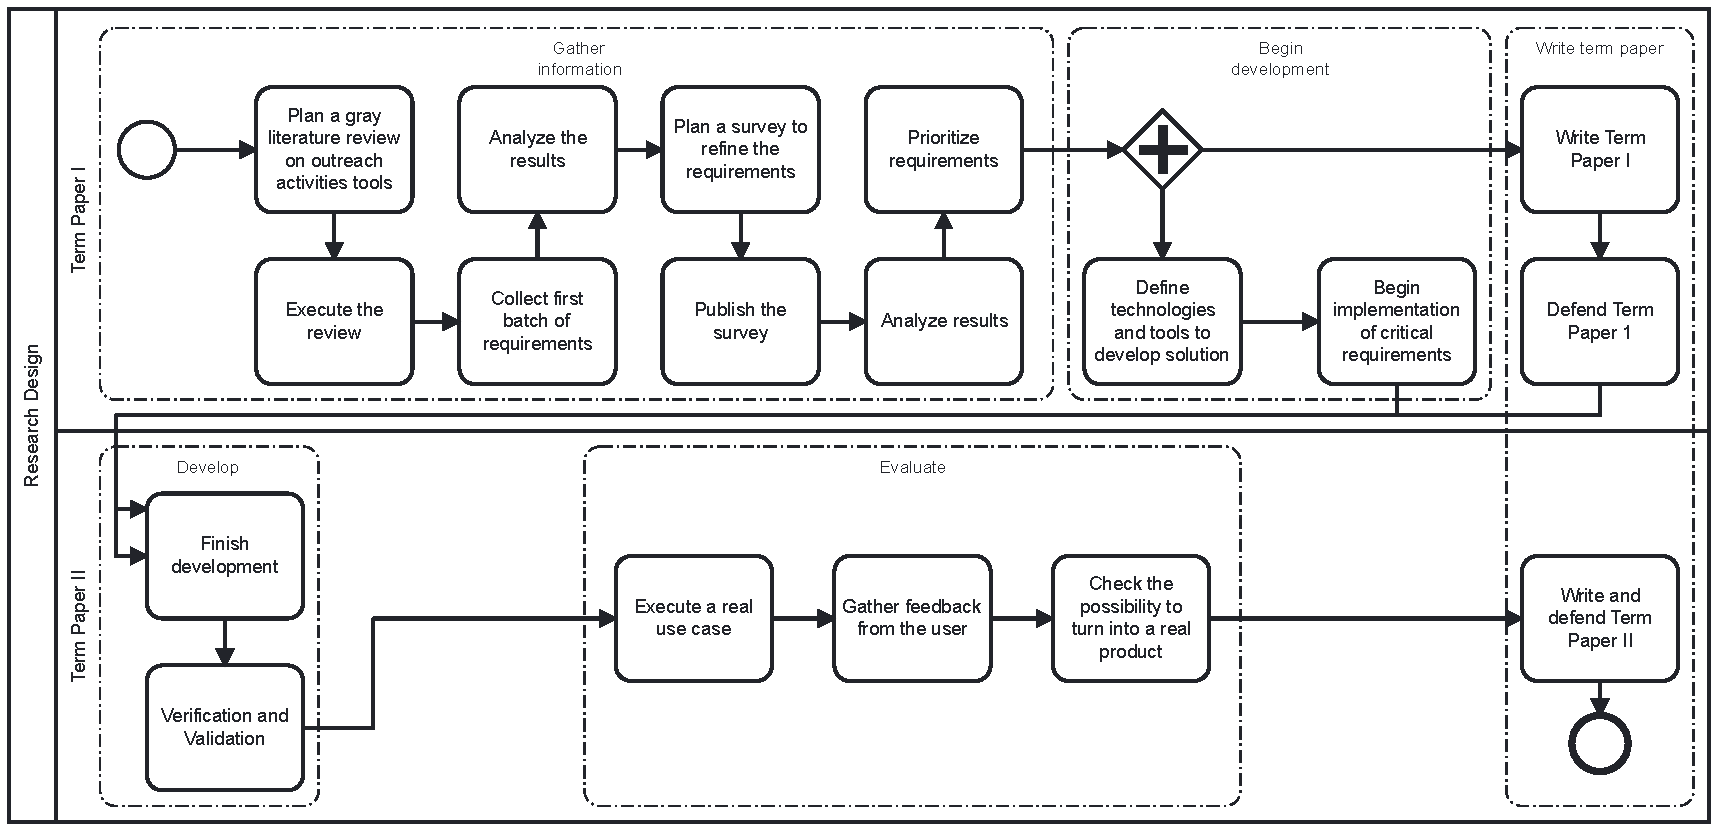
\includegraphics[width=11cm, ]{img/2-research design.pdf}
  \end{figure}
\end{frame}

% \item Contexto
% 	        \SubItem{Curricularização da extensão}
% 	        \SubItem{Resoluções}
% 	        \SubItem{Unipampa Cidadã}
%---------------------------------------------------------------------
\section{Contexto}
\subsection*{Contexto}
%---------------------------------------------------------------------

%######################################################################
\begin{frame}{{\sffamily Curricularização da Extensão}}
  \begin{block}{Legislação}
    \begin{itemize}
      \item Política Nacional de Extensão Universitária %Garantir q extensão pode resolver qualquer problema social, promover solidariedade tanto nacional como internacionalmente, reconhecer que extensão é uma peça essencial em universidades publicas;
            \SubItem{Extensão como solução para problemas sociais}
            \SubItem{Extensão como ferramenta essencial}
            \SubItem{Promover solidariedade e conscientização ambiental}
      \item Parte do curso como extensão (Res. 7 de 2018) %10% de horas, aumenta a procura e demanda
            \SubItem{10\% de horas do total}
            \SubItem{Adaptação em até 3 anos}
    \end{itemize}
  \end{block}
\end{frame}

\begin{frame}{{\sffamily Curricularização da Extensão na UNIPAMPA}}
  \begin{block}{Resoluções}
    \begin{itemize}
      \item Objetivos da extensão pela Res. 317 de 2021
            \SubItem{Desenvolver a educação crítica, cívica, interdisciplinar e responsável}
            \SubItem{Fortalecer o vínculo entre ensino, pesquisa e extensão}
      \item Formalização pela Res. 332 de 2021
            \SubItem{Órgãos gestores, participantes da extensão, tramitações}
      \item Cadeira de Resolução de Problemas
    \end{itemize}
  \end{block}
\end{frame}
%######################################################################

%######################################################################
\begin{frame}{{\sffamily Programas e projetos de extensão}}
  % Objetivo não é criar um laço de dependência entre comunidades, so para resolver um determinado problema e deixar que eles consigam andar com as proprias pernas depois, por isso a qualidade
  \begin{block}{O que são}
    Ações que envolvem ensino, pesquisa e a comunidade externa.
    \begin{itemize}
      \item Projetos possuem um objetivo específico e prazos determinados
      \item Um programa é um conjunto de projetos % Da pra falar das roles
    \end{itemize}
  \end{block}

  \begin{block}{Exemplos de programas}
    \begin{itemize}
      \item Programa C
      \item Programa JEDI
      \item Programa TRAMAS
    \end{itemize}
  \end{block}

\end{frame}

\begin{frame}{{\sffamily Unipampa Cidadã}}
  \begin{block}{}
    \begin{itemize}
      \item Extensão curricular
      \item Atividades solidárias % , 
            \SubItem{Campanha do agasalho, arrecadação de alimentos, suporte a asilos}
      \item Formação de egressos mais socialmente responsáveis % Egressos mais consientes com a responsabilidade social
      \item Oferecida por todos os cursos % 60 and a maximum of 120 hours
            \SubItem{Mínimo de 60 e máximo de 120 horas}
      \item Formulário de finalização da atividade.
    \end{itemize}
  \end{block}
\end{frame}
%######################################################################

\section{Literatura Cinza}
\subsection*{Literatura Cinza}

\begin{frame}{{\sffamily Literatura Cinza}}
  \begin{block}{Motivação}
    \begin{itemize}
      \item Poucos resultados na literatura branca
      \item Na maioria das vezes ferramentas não possuem artigo publicado
    \end{itemize}
  \end{block}

  \begin{block}{Objetivos}
    \begin{itemize}
      \item Analisar ferramentas semelhantes ao MVP
            \SubItem{Funcionalidades e detalhes em comum}
      \item Extrair uma lista preliminar de requisitos
    \end{itemize}
  \end{block}
  Conduzido por dois alunos: Igor Costa e Lucas Fell.
\end{frame}

\begin{frame}{{\sffamily Questões de Pesquisa}}
  \begin{table}[!htb]
  \centering
  \label{tab:research-questions}
  \footnotesize
  \begin{tabular}{l|p{9cm}}
    \bottomrule
    \rowcolor[rgb]{0.753,0.753,0.753} \multicolumn{1}{c|}{\textbf{ID}} & \multicolumn{1}{c}{\textbf{Questão}}                                                                        \\
    \hline
    \rowcolor[rgb]{0.898,0.898,0.898} QP 1                             & Quais ferramentas existem atualmente que realizam gestão acadêmica?                                         \\
    QP 1.1                                                             & Quais delas possuem funcionalidades relacionadas ou dão suporte à atividades de extensão?                   \\
    \rowcolor[rgb]{0.898,0.898,0.898} QP 1.2                           & Quais são as funcionalidades disponibilizadas por essas ferramentas?                                        \\
    QP 1.3                                                             & Quais são as funcionalidades mais comuns entre este tipo de ferramenta?                                     \\
    \rowcolor[rgb]{0.898,0.898,0.898} QP 1.4                           & Quais dados as ferramentas usam em relação às atividades, cadastro de participantes e cadastro de usuários? \\
    \toprule
  \end{tabular}
\end{table}
\end{frame}

\begin{frame}{{\sffamily Critérios de Inclusão}}
  \begin{block}{Duas etapas}
    \begin{enumerate}
      \item Diferenciação de ferramentas e catálogos
            \SubItem{Login, inscrição em atividades}
      \item Aplicação dos critérios de inclusão
    \end{enumerate}
  \end{block}
  \begin{table}[!htb]
  \centering
  \caption{Inclusion Criteria}
  \label{tbl:gl-inclusion-criteria}
  \footnotesize
  \begin{tabular}{c|l}
    \bottomrule
    \rowcolor[rgb]{0.753,0.753,0.753} \textbf{ID} & \multicolumn{1}{c}{\textbf{Inclusion Criteria}}                     \\
    \hline
    \rowcolor[HTML]{DEDEDE}
    IC 1.                                         & The tool or website supports the management of outreach activities. \\
    IC 2.                                         & The tool or website has a stable version.                           \\
    \rowcolor[HTML]{DEDEDE}
    IC 3.                                         & If it is a tool, it must have documentation.                        \\
    \toprule
  \end{tabular}
  \fonte{Author.}
\end{table}
\end{frame}

\begin{frame}{{\sffamily Critérios de Exclusão}}
  \begin{block}{Critérios de exclusão}
    Qualquer resultado que se encaixa em apenas um é automaticamente excluído.
  \end{block}
  \begin{table}
  \centering
  \caption{Exclusion Criteria}
  \label{tbl:gl-exclusion-criteria}
  \resizebox{\textwidth}{!}{
    \begin{tabular}{|c|l|}
      \hline
      \rowcolor[rgb]{0.753,0.753,0.753} ID & \multicolumn{1}{c|}{Exclusion Criteria}                                                                   \\
      \hline
      EC 1.                                & If it is a tool, it does not have a source code download or an online page.                               \\
      \hline
      EC 2.                                & The tool or the website has not received updates for more than 10 years.                                  \\
      \hline
      EC 3.                                & The tool or website is for the exclusive use of the organization, that is, closed to the external public. \\
      \hline
      EC 4.                                & The tool or website is paid and does not provide a trial version or all outreach activities are paid.     \\
      \hline
    \end{tabular}
  }
  \fonte{Author.}
\end{table}
\end{frame}

\begin{frame}{{\sffamily Critérios de Qualidade}}
  \begin{block}{Atende ao critério?}
    Sim (1); Parcialmente (0.5); Não (0).
  \end{block}
  \begin{table}[!htb]
  \centering
  %   \caption{Quality Criteria}
  %   \label{tbl:gl-quality-criteria}
  \arrayrulecolor{black}
  \tiny
  \begin{tabular}{c|p{3.5cm}|p{1.5cm}|p{1.5cm}|p{2cm}}
    \bottomrule
    \rowcolor[rgb]{0.753,0.753,0.753} {\cellcolor[rgb]{0.753,0.753,0.753}}                              & \multicolumn{1}{c|}{{\cellcolor[rgb]{0.753,0.753,0.753}}}                                                  & \multicolumn{3}{c}{\textbf{\textbf{Pontuação}}}                                                                                                           \\
    \hhline{>{\arrayrulecolor[rgb]{0.753,0.753,0.753}}-->{\arrayrulecolor{black}}---}
    \rowcolor[rgb]{0.753,0.753,0.753} \multirow{-2}{*}{{\cellcolor[rgb]{0.753,0.753,0.753}}\textbf{ID}} & \multicolumn{1}{c|}{\multirow{-2}{*}{{\cellcolor[rgb]{0.753,0.753,0.753}}\textbf{Critérios de Qualidade}}} & \multicolumn{1}{c|}{\textbf{Sim (1)}}           & \multicolumn{1}{c|}{\textbf{Parcial. (0.5)}} & \multicolumn{1}{c}{\textbf{Não (0)}}                     \\
    \hline
    \rowcolor[rgb]{0.898,0.898,0.898} CQ 1.                                                             & A ferramenta usa uma quantidade relevante de dados relacionados às atividades de extensão?                 & A ferramenta usa 20 ou mais                     & Usa de 10 a 19                               & Usa 10 dados ou menos                                    \\
    CQ 2.                                                                                               & A ferramenta possui funcionalidades exclusivos entre as ferramentas selecionadas?                          & A ferramenta possui mais que 1                  & Possui 1                                     & Nenhuma funcionalidade exclusiva                         \\
    \rowcolor[rgb]{0.898,0.898,0.898} CQ 3.                                                             & A ferramenta possui uma quantidade relevante de funcionalidades entre as coletados?                        & A ferramenta possui 14 ou mais                  & De 9 até 13                                  & Possui 8 funcionalidades em comum com outras ferramentas \\
    \multicolumn{1}{l|}{CQ 4.}                                                                          & A ferramenta tem suporte especializado?                                                                    & Sim                                             & Parcialmente                                 & Não                                                      \\
    \rowcolor[rgb]{0.898,0.898,0.898} \multicolumn{1}{l|}{CQ 5.}                                        & A ferramenta foi mantida com frequência?                                                                   & A última atualização foi em 2022                & Foi de 2021 até 2019                         & Foi em 2018 ou antes                                     \\
    \toprule
  \end{tabular}
\end{table}
\end{frame}

\begin{frame}{{\sffamily Condução}}
  % Divisão de trabalho
  % Período de tempo
  % Alteração nas strings
  \begin{block}{Divisão de trabalho}
    \begin{itemize}
      \item Dividido igualmente entre os dois autores
      \item Cada um analisou 500 resultados no total
    \end{itemize}
  \end{block}
  \begin{block}{Período de tempo}
    Entre 17/02/2022 e 20/02/2022.
  \end{block}
  \begin{block}{Strings alteradas}
    \begin{itemize}
      \item -SIGAA
      \item site:.edu.br
    \end{itemize}
  \end{block}
\end{frame}

\begin{frame}{{\sffamily Resultados}}
  % 169 encontradas e 12 depois 
  \begin{block}{Ferramentas encontradas}
    169 no total e 12 depois da aplicação dos critérios.
  \end{block}
  \begin{table}
  \centering
  \caption{Search Results}
  \label{tbl:gl-search-results}
  \scriptsize
  \begin{tabular}{c|p{6cm}|l|p{1.5cm}|c}
    \bottomrule
    \rowcolor[rgb]{0.753,0.753,0.753} \textbf{No.} & \multicolumn{1}{c|}{\textbf{Search String}}                                                                                 & \textbf{Evaluated Results}  & \textcolor[rgb]{0.137,0.137,0.145}{\textbf{Potential New Tools}} & \textbf{Total} \\
    \hline
    \rowcolor[rgb]{0.898,0.898,0.898} 1            & sistema gestão acadêmicas (atividades \textbar{} projetos) site:.edu.br                                                     & 100 out of $\sim$1.250.000  & 4                                                                & 4              \\
    2                                              & (sistema \textbar{} ferramenta) gestão acadêmicas (atividades \textbar{} projetos) extensão site:.edu.br -SIGAA             & 100 out of $\sim$182.000    & 11                                                               & 15             \\
    \hhline{>{\arrayrulecolor[rgb]{0.898,0.898,0.898}}->{\arrayrulecolor{black}}->{\arrayrulecolor[rgb]{0.898,0.898,0.898}}---}
    \rowcolor[rgb]{0.898,0.898,0.898} 3            & (ferramenta \textbar{} aplicação) extensão (programa \textbar{} projeto) (gestão \textbar{} gerenciamento) -SIGAA           & 100 out of $\sim$15.600.000 & 9                                                                & 24             \\
    4                                              & (app \textbar{} aplicativo) extensão (programa \textbar{} projeto) (administração \textbar{} gerência) -SIGAA               & 100 out of $\sim$7.140.000  & 13                                                               & 37             \\
    \rowcolor[rgb]{0.898,0.898,0.898} 5            & ferramenta extensão (programa \textbar{} projeto) (gestão \textbar{} gerência) -SIGAA                                       & 100 out of $\sim$11.000.000 & 27                                                               & 64             \\
    6                                              & (ferramenta \textbar{} aplicação \textbar{} app \textbar{} aplicativo) extensão (programa \textbar{} projeto) gestão -SIGAA & 100 out of $\sim$22.500.000 & 15                                                               & 79             \\
    \rowcolor[rgb]{0.898,0.898,0.898} 7            & software extensão (programa \textbar{} projeto) (gerência \textbar{} gestão \textbar{} controle) -SIGAA                     & 100 out of $\sim$8.300.000  & 24                                                               & 103            \\
    8                                              & (software \textbar{} ferramenta \textbar{} aplicação) extensão atividade -SIGAA                                             & 100 out of $\sim$30.900.000 & 10                                                               & 113            \\
    \rowcolor[rgb]{0.898,0.898,0.898} 9            & sistema extensão (projeto \textbar{} programa \textbar{} atividade) gestão -SIGAA                                           & 100 out of $\sim$26.400.000 & 30                                                               & 143            \\
    10                                             & acadêmica extensão (projeto \textbar{} programa \textbar{} atividade) -SIGAA                                                & 100 out of $\sim$17.000.000 & 26                                                               & 169            \\
    \arrayrulecolor{black}\toprule
  \end{tabular}
  \fonte{Author.}
\end{table}
\end{frame}

\begin{frame}{{\sffamily Resultados}}
  % 37 funcionalidades algumas mescladas
  % SIGAA e CAEX mais pontuação
  \begin{block}{Funcionalidades encontradas}
    \begin{itemize}
      \item 37 no total, entre todas as ferramentas analisadas
      \item SIGAA e CAEX com a maior pontuação
    \end{itemize}
  \end{block}
  \begin{table}
  \centering
  \resizebox{\linewidth}{!}{%
    \arrayrulecolor{black}
    \begin{tabular}{lc|c|c|c|c|l}
      \bottomrule
      \multirow{3}{*}{~}                                                                                        & \multicolumn{6}{c}{{\cellcolor[rgb]{0.753,0.753,0.753}}\textbf{Critérios de Qualidade}}                                                                                                                                                                                                                                                                                                \\
                                                                                                                & {\cellcolor[rgb]{0.753,0.753,0.753}}\textbf{CQ 1.}                                      & {\cellcolor[rgb]{0.753,0.753,0.753}}\textbf{CQ 2.} & {\cellcolor[rgb]{0.753,0.753,0.753}}\textbf{CQ 3.} & {\cellcolor[rgb]{0.753,0.753,0.753}}\textbf{CQ 4.} & {\cellcolor[rgb]{0.753,0.753,0.753}}\textbf{CQ 5.} & {\cellcolor[rgb]{0.753,0.753,0.753}}                                     \\
                                                                                                                & {\cellcolor[rgb]{0.753,0.753,0.753}}\textbf{Pont.}                                      & {\cellcolor[rgb]{0.753,0.753,0.753}}\textbf{Pont.} & {\cellcolor[rgb]{0.753,0.753,0.753}}\textbf{Pont.} & {\cellcolor[rgb]{0.753,0.753,0.753}}\textbf{Pont.} & {\cellcolor[rgb]{0.753,0.753,0.753}}\textbf{Pont.} & \multirow{-2}{*}{{\cellcolor[rgb]{0.753,0.753,0.753}}\textbf{Resultado}} \\
      \hline
      \multicolumn{1}{l|}{{\cellcolor[rgb]{0.753,0.753,0.753}}\textbf{CAEX}}                                    & 0,0                                                                                     & 1,0                                                & 1,0                                                & 1,0                                                & 1,0                                                & \multicolumn{1}{c}{4,0}                                                  \\
      \rowcolor[rgb]{0.898,0.898,0.898} \multicolumn{1}{l|}{{\cellcolor[rgb]{0.753,0.753,0.753}}\textbf{SIGAA}} & 1,0                                                                                     & 0,5                                                & 1,0                                                & 1,0                                                & 1,0                                                & \multicolumn{1}{c}{4,5}                                                  \\
      \toprule
    \end{tabular}
  }
\end{table}

  % Respostas as questões de pesquisa
  % Ajuda 
  % (QP1) Resultados que passaram no CI1.
  % (QP1.1, QP1.2, QP1.3) Matriz de funcionalidades
  % (QP1.4) Segunda extração de dados
\end{frame}
% Survey - lista preliminar da literatura -> validação com usuários reais, agregando novos requisitos
% protocolo, questionário, requisitos propostos, resultados, análise

%==============================================================================
\chapter{Survey}\label{survey}
%==============================================================================

\section{Survey protocol}\label{sec:sv-p}

\subsection{Pilot questionnaire}\label{sec:sv-p:pilot}

As \citeonline[p. 75]{kasunic2005designing} describes, a pilot test is a simulation of the real questionnaire carried out with a small number of members from the target audience. For this, the authors hand picked 7 (seven) people, out of which 4 (four) were students, 2 (two) were professors and 1 (one) was an \acl{TAE} (\ac{TAE}). The reason behind choosing this specific number of respondents is due to the following:
\begin{inparaenum}[(i)]
  \item All defined profiles for the respondents were chosen and
  \item the ratio of 4/2/1 is aligned with the expected numbers of submitted questionnaires per profile.
\end{inparaenum}

Unfortunately, the person chosen for the third profile, \ac{TAE}, wasn't able to answer. However, even though there are 3 (three) profiles, the questionnaire itself only has 2 (two) tracks of questions, one for students and the other for professors/\acp{TAE}. Because of that, the consequences of this happening weren't too impactful.

As for the pilot results, a lot of great feedback was received, along with some compliments on the organization of the questionnaire. There were issues with the person identification section, where the age was changed from a number to a range of numbers, such as between 21-29 years old.

\subsection{Distribute the Questionnaire}\label{sec:survey-distribute}

\section{Threats to validity}\label{sec:sv-validity}

% TAE didn't answer pilot test

\section{Results}\label{sec:sv-results}

\section{MVP}
\subsection*{MVP}

\begin{frame}{{\sffamily Análise e Projeto do MVP}}
  \begin{block}{Perfis de Usuário}
    \begin{itemize}
      \item Participante
      \item Instrutor
      \item Proponente
      \item Coordenador
      \item Supervisor

      \item Participante Externo
    \end{itemize}
  \end{block}
\end{frame}

\begin{frame}{{\sffamily Casos de Uso}}
  \begin{figure}
    \vfill
    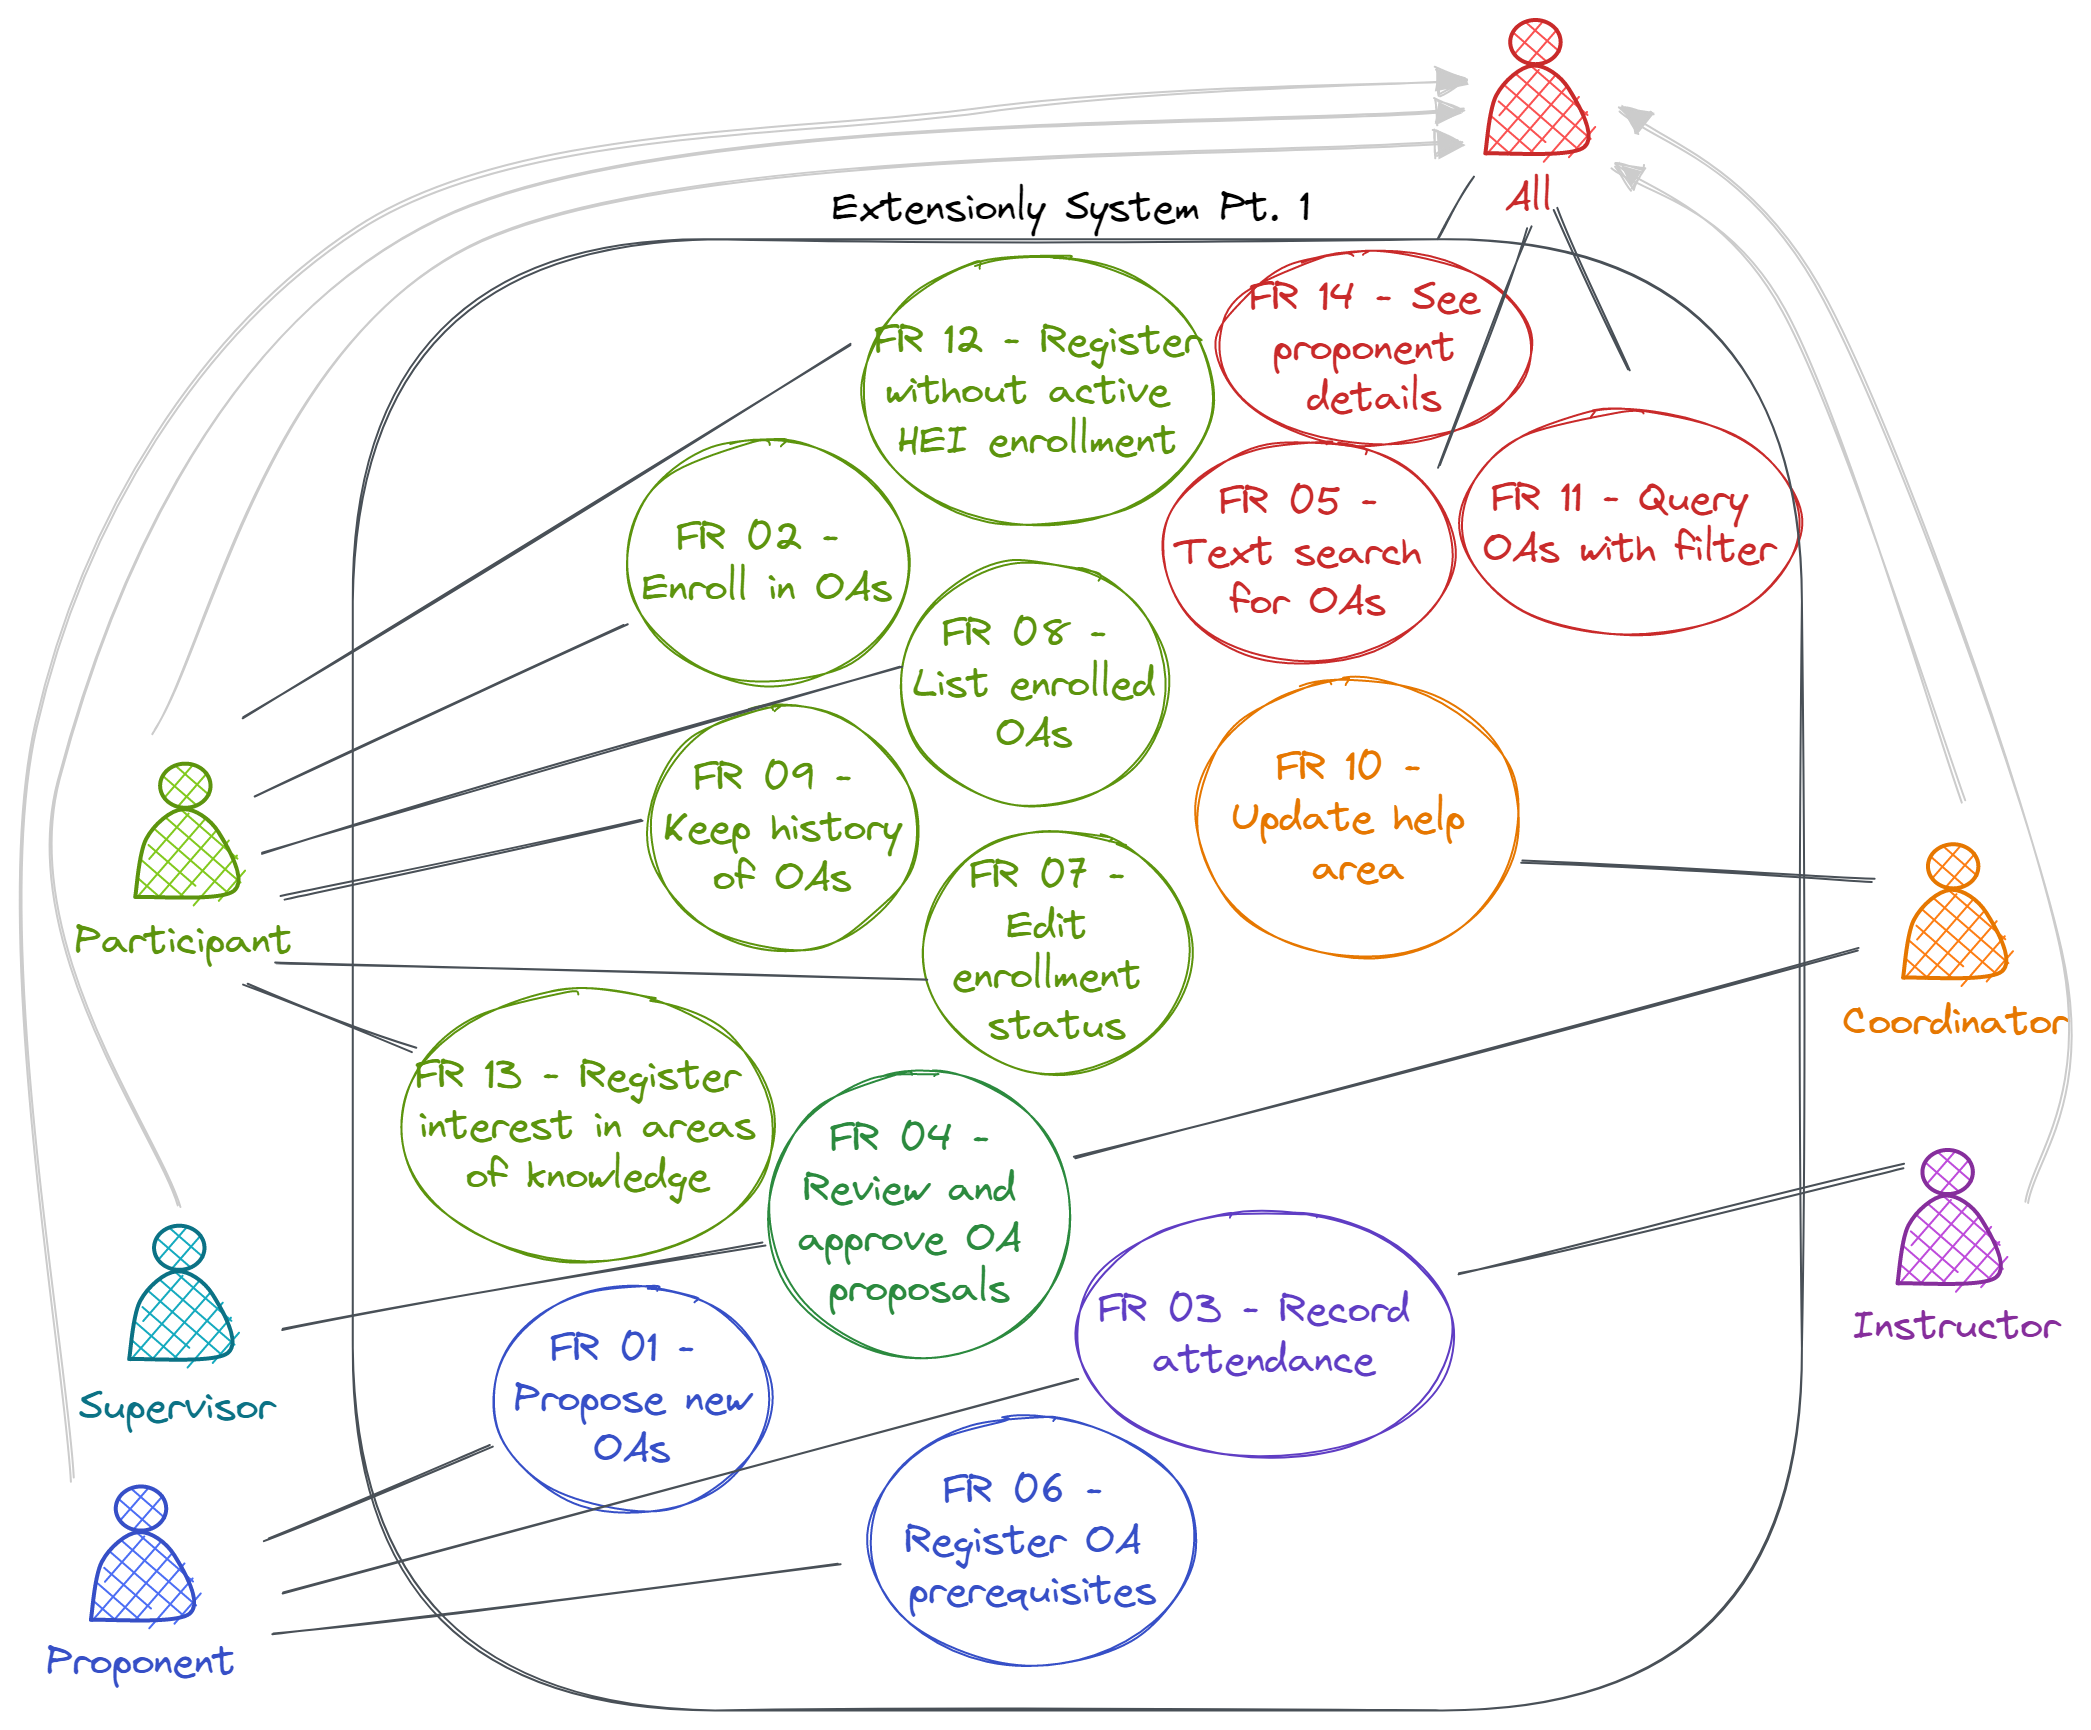
\includegraphics[width=7.5cm, ]{imagens/6-use-case-1.png}
    \vfill
  \end{figure}
\end{frame}

\begin{frame}{{\sffamily Casos de Uso}}
  \begin{figure}
    \vfill
    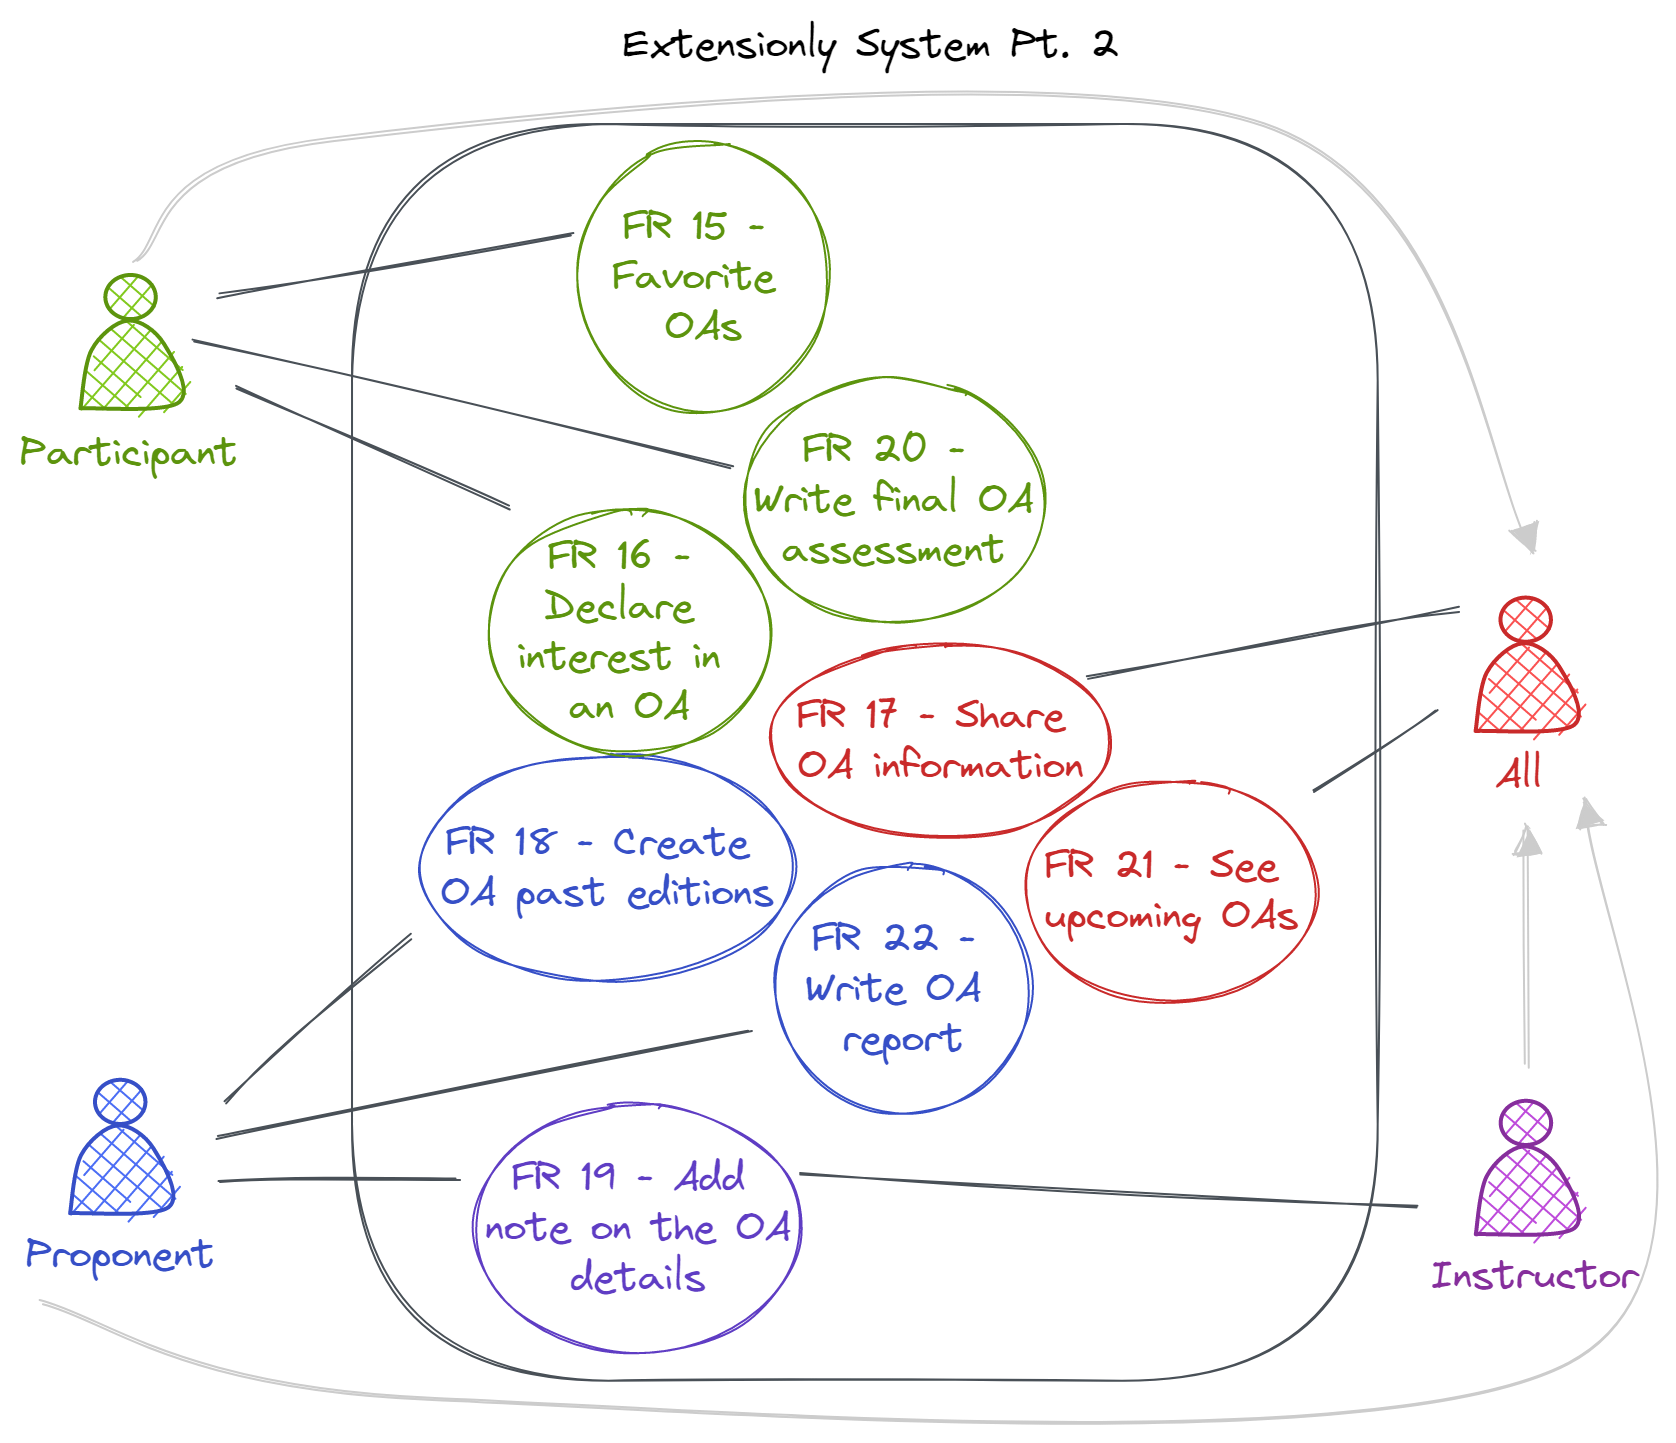
\includegraphics[width=7.5cm, ]{imagens/6-use-case-2.png}
    \vfill
  \end{figure}
\end{frame}

\begin{frame}{{\sffamily Análise e Projeto do MVP}}
  \begin{block}{Decisões de Projeto}
    \begin{itemize}
      \item Linguagem de programação:
            \SubItem{TypeScript}
      \item Framework:
            \SubItem{React com NextJS}
      \item Arquitetura:
            \SubItem{Componentes, reusabilidade}
            \SubItem{SSR, SEO}
      \item Multi idiomas:
            \SubItem{Português e Inglês inicialmente}
    \end{itemize}
  \end{block}
\end{frame}
\begin{frame}{{\sffamily Análise e Projeto do MVP}}
  \begin{block}{Decisões de Projeto}
    \begin{itemize}
      \item Estatísticas Transparentes:
            \SubItem{Privacidade x Entender o uso da ferramenta}
            \SubItem{Dados anônimos}
            \SubItem{Plausible}
    \end{itemize}
  \end{block}
\end{frame}

\begin{frame}{{\sffamily Arquitetura}}
  \begin{figure}
    \vfill
    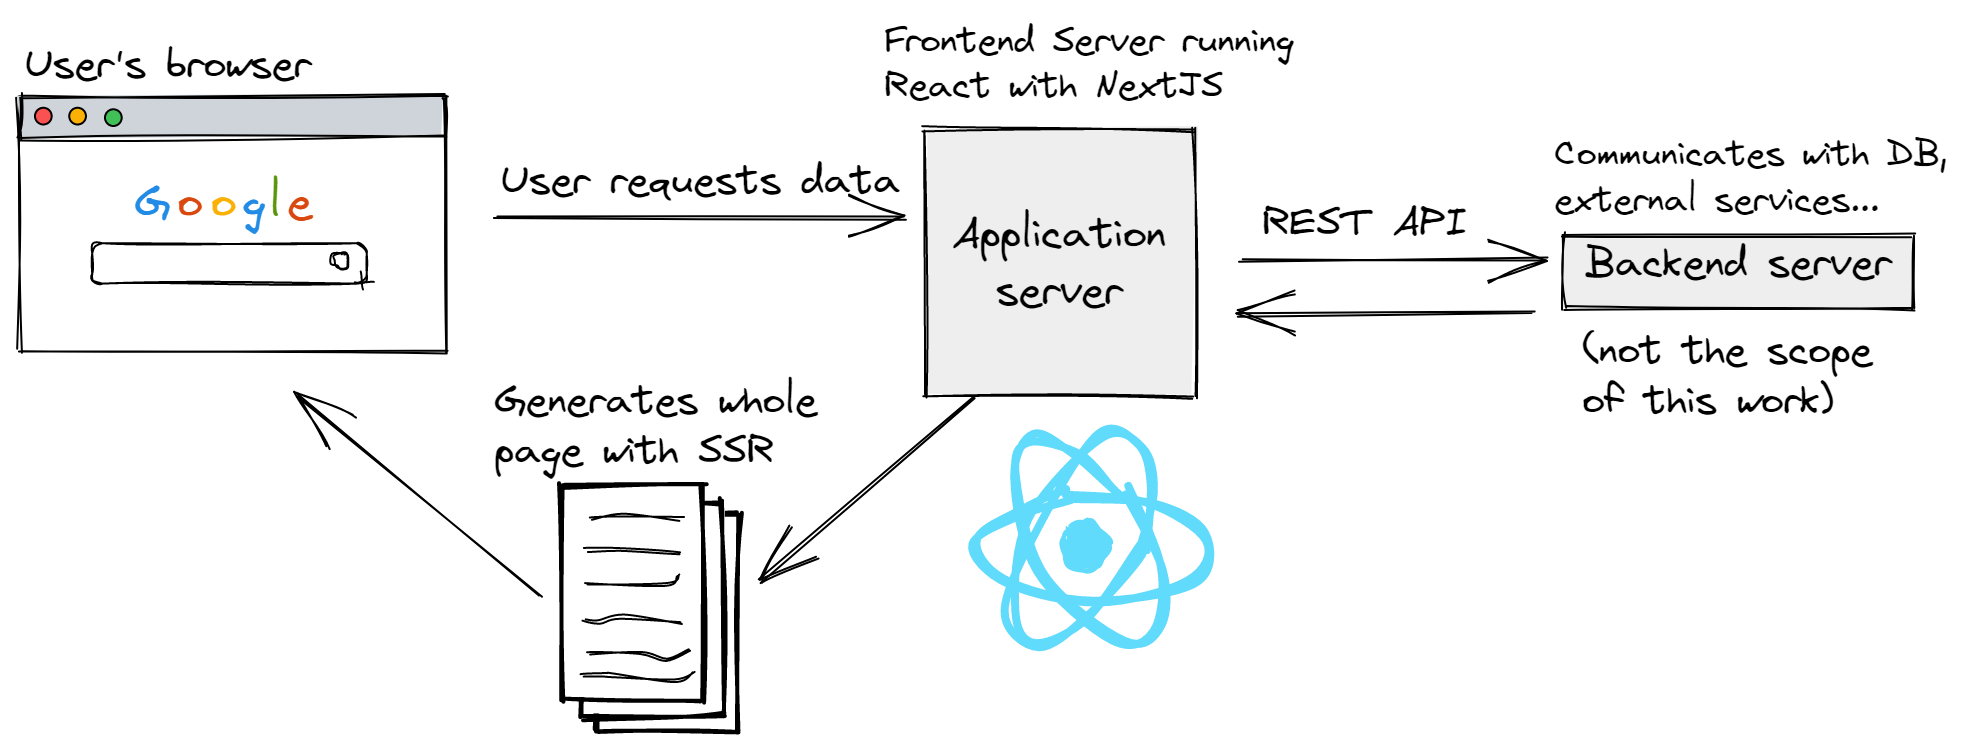
\includegraphics[width=10.5cm, ]{imagens/6-architecture.png}
    \vfill
  \end{figure}

\end{frame}

% Considerações Preliminares - possível publicação em eventos da área, com os resultados encontrados (ERES agosto), mais eventos (SBIE), artigos relacionados à extensão
%==============================================================================
\chapter{Preliminary Considerations}\label{conclusao}
%==============================================================================

% Em Trabalhos de Conclusão de Curso, use ``\emph{Considerações Finais}'' e não ``\emph{Conclusão}''.

% Bom trabalho!

The goal of the current work was to thoroughly examine the administration of \aclp{OA} in order to create a tool that supports the administrative procedures, makes it easier to communicate with the outside world, and improves student participation and dissemination. For this, two artifacts were produced: a review of the gray literature to locate comparable solutions already in use, eliciting their critical features, and a survey of potential end users of the tool to order the requirements by importance and gather additional ideas on the topic.

Five particular goals were established in order to accomplish the overall goal of the work, which is to create the tool's front end to support the management of \ac{UNIPAMPA}'s outreach programs and projects. They were previously described in \Cref{sec:objectives}.

The first goal was to conduct a review of the gray literature to look for features in tools that were similar to what is being proposed. Based on the results, it is clear that this goal was accomplished, as it was possible to identify a number of tools and, in the end, to produce a list of tools that was significant in size, complete with their functionalities and specific information, which was especially helpful in planning.

The second goal relates to the development of a survey to ascertain the viewpoints of potential end users. This goal was accomplished since it was feasible to examine the problems and worries that users had, which made it possible to draw out a number of enhancements and features for the suggested tool.

The third particular goal is the creation of a development roadmap and tangible tasks. This goal was only partially attained because the transition from \ac{FR} to development tasks won't take place until the second phase of this work's development, or \ac{TP} II.

The fourth goal is to research, evaluate, and select a development stack, including a programming language, an architecture, and a framework, for the front end of the suggested tool. This goal was accomplished; prior decisions were presented earlier in \Cref{extensionly}.

The creation of a \ac{MVP} for the tool's front end is the fifth and final specific goal, and it has not yet been accomplished because the tool's development is still on the horizon.

The hypothesis of this work, which can't yet be confirmed or disproved because the application hasn't yet been developed and tested with end users, is that "With a tool to support the management of outreach programs and projects, it's possible to have a reduction on the effort needed to create an outreach activity and an increase in the engagement of volunteer outreach participants." However, given all of the good feedback that the survey respondents supplied, it is extremely probable that this theory will be proven with the accurate and thorough development of the application.

With a tool of this kind, it is feasible to lessen the manual and repetitive work required in the registration of new proposals for outreach efforts, facilitating operations like generating certificates more effectively. This is the research question of this work, described in \Cref{tbl:intro-objectives}. Additionally, students will know where to go if they need assistance with the subject thanks to a platform that centralizes information about university outreach, which will increase the dissemination of new initiatives. With the use of the technology, the connection between the teacher and the participant will also be reinforced, enabling richer interactions and experiences for both parties.

The survey's results gave the researchers insight into what potential end users could think about the presence of a tool like this to help them with related tasks. It allowed for the reevaluation of various implementation-related difficulties while taking into consideration suggestions made. It is safe to state that without a study of these users' opinions, the tool would be in serious danger of not meeting of the previously established expectations.

A lot of effort will be devoted to the application's development for the second iteration of this \ac{TP} so that real-world use case scenarios involving professors and students can be tested. The goal is to demonstrate the tool's value to the university as a whole by integrating its capabilities into actual outreach initiatives and projects from \ac{UNIPAMPA}.

\begin{frame}[plain,t]
  \titlepage
\end{frame}

\end{document}